\subsubsection{FC Portugal} \label{fc_portugal}

Portugalský tím FC Portugal\cite{fc_portugal}.
Navrhli metódu pre kopanie do viacerých smerov. Je zložený z troch častí. Prvou je vytvorenie dráhy, akou musí smerovať noha robota, aby sa lopta dostala do želaného smeru. Na vytvorenie krivky pohybu nohy použili Bezierovu rovnicu tretieho stupňa. Druhou časťou je modul pre inverznú kinematiku, ktorý na základe predtým vypočítanej krivky vypočíta natočenie kĺbov pre vykonanie kopu. Posledná časť je stabilizačný modul, ktorý sa snaží dosiahnuť to, aby sa ťažisko robota nachádzalo v ploche druhej podpornej nohy. Do fázy stabilizovania vstupujú aj horné končatiny, ktoré sa upažia alebo predpažia. V extrémnom prípade, ak nestačí pohybovanie rukou, upravuje sa pozícia bokov, členkov a robot sa predkláňa na vyrovnanie stability. %Vo výsledkoch boli úspešní pri vypočítavaní krivky (jednoduchý matematický výpočet). Taktiež výsledky dosiahli, že robot kopol loptu do požadovaného smeru. Očakávania nenaplnili pri dosahovaní stability kopu. Neriešili parametrizovanie vzdialenosti.

\begin{figure}[H]
	\center
	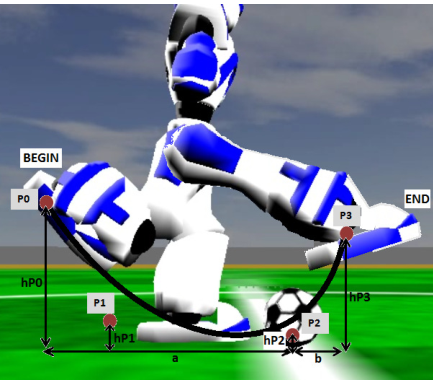
\includegraphics[scale=1]{./data/kick_arch_fc_portugal}
	\caption{Schéma kopu FC Portugal \cite{fc_portugal}}
	\label{pic_kick_arch_fc_portugal}
\end{figure}